Anteriormente, en la sección ``\nameref{especificacion_plan_pruebas}'' perteneciente al capítulo \ref{chapter04} se explicó que tendrían lugar una serie de pruebas de rendimiento sobre el Punto de Entrada de Datos del sistema.  En esta sección se detallará la metodología seguida para la realización de dichas pruebas así como los resultados obtenidos sobre las mismas.


\subsection{Proceso y ámbito de las mediciones}
\label{pruebas:proceso_ambito_mediciones}
	En la sección ``\nameref{definicion_sistema}'', también del capítulo \ref{chapter04} se indicó que sólo forma parte del alcance de éste proyecto la creación de un servicio de generación de SQL como parte del Punto de Entrada de Datos.  Debido a esto y con el fin de aislar las mediciones a un ámbito relevante para ésta documentación, éstas han sido realizadas con los servicios de generación de RDF y CKAN desactivados.
	
	Las mediciones tendrán lugar mediante el envío de un fichero XML al Punto de Entrada de Datos para su procesado e inserción en base de datos usando el parser común y el servicio de generación de SQL.  Para hacer las mediciones lo más exactas posible se repetirán un total de tres veces y posteriormente se calculará la mediana.  Con el fin de evitar interferencias externas, cada medición se realizará sobre una base de datos MySQL\footnote{La versión de MySQL utilizada durante las mediciones es la 5.5.37} vacía y un servicio Apache\footnote{La versión de Apache utilizada durante las mediciones es la 2.4.7} recién iniciado.
	
	Las herramientas utilizadas para medir realizar las mediciones son el módulo \textit{memory profiler}\footnote{El módulo \textit{memory profiler} puede descargarse en \url{https://pypi.python.org/pypi/memory_profiler}} para la medición del rendimiento espacial, y el comando \textit{time}\footnote{El comando \textit{time} forma parte de los sistemas tipo UNIX y permite medir la duración de la ejecución de un determinado programa} para la medición del rendimiento temporal.  Las mediciones de espacio y tiempo se realizarán en ejecuciones diferentes para que no interfieran entre sí.
	

\subsection{Resultado de las mediciones}
	A continuación se expondrán los resultados obtenidos de las mediciones.  
	
	Las figuras \ref{fig:obs_vs_tiempo}, \ref{fig:obs_segundo} y  \ref{fig:obs_vs_memoria} muestran respectivamente el número de observaciones del catálogo de datos entrante frente al tiempo de procesado del mismo, el número de observaciones procesadas por segundo y el consumo de memoria del Punto de Entrada de Datos durante el procesado.  Los datos utilizados para la creación de dichas figuras pueden consultarse con mayor detalle en el anexo \ref{anexo:resultados_mediciones}.
	
	\begin{figure}[h]
		\centering
		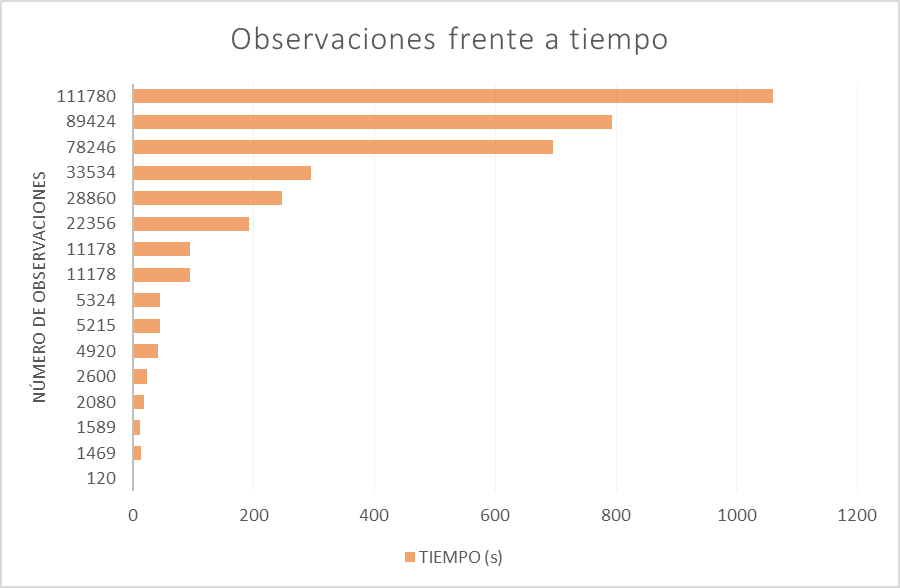
\includegraphics[width=0.8\textwidth]{mediciones/obs_vs_tiempo}
		\caption{Número de observaciones entrantes frente a tiempo de procesado}
		\label{fig:obs_vs_tiempo}
	\end{figure}
	
	\begin{figure}[h]
		\centering
		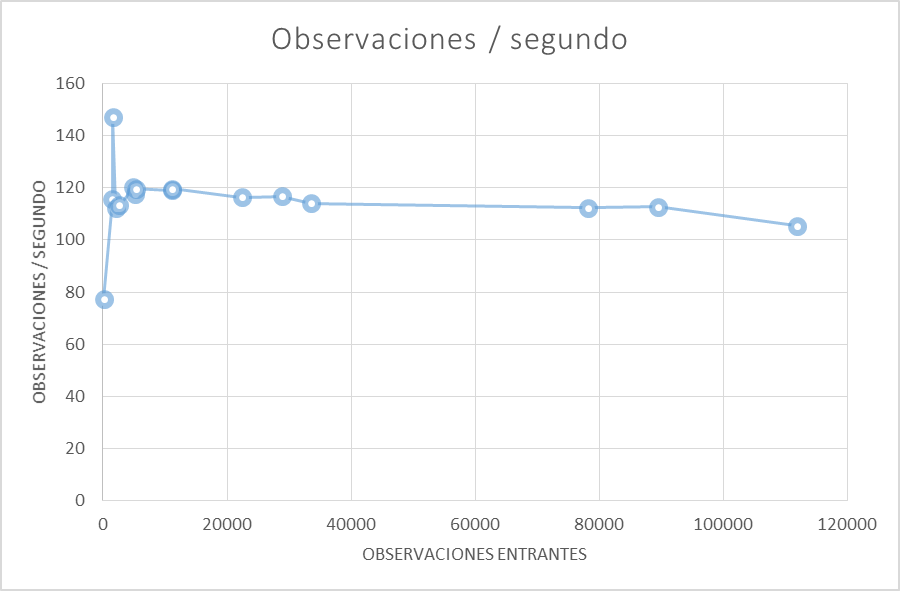
\includegraphics[width=0.8\textwidth]{mediciones/observaciones_segundo}
		\caption{Número de observaciones por segundo procesadas}
		\label{fig:obs_segundo}
	\end{figure}
	
	\begin{figure}[h]
		\centering
		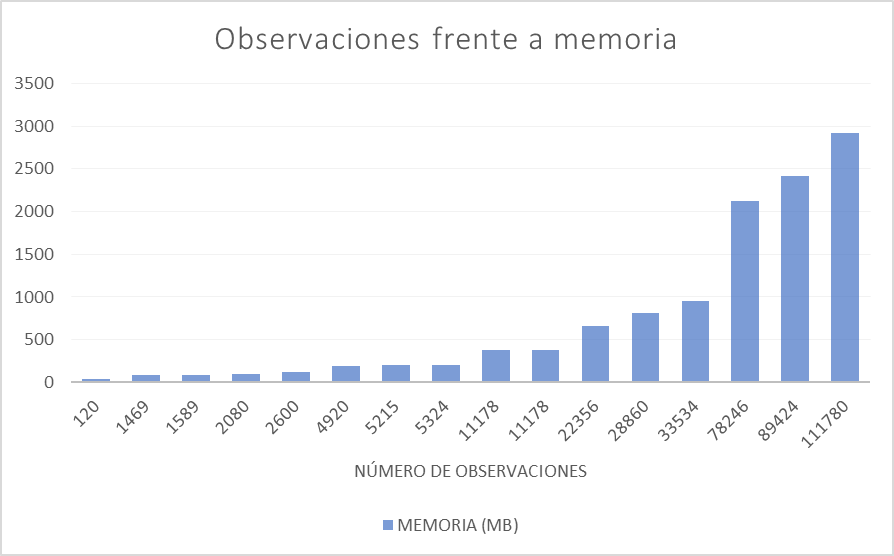
\includegraphics[width=0.8\textwidth]{mediciones/obs_vs_memoria}
		\caption{Número de observaciones frente a memoria durante el procesado}
		\label{fig:obs_vs_memoria}
	\end{figure}	
	 

\subsection{Análisis de los resultados}
	A continuación se expondrán las conclusiones extraídas de los resultados obtenidos durante las mediciones. Los resultados han sido expuestos en la tabla \ref{table:mediciones_receiver} y las figuras \ref{fig:obs_vs_tiempo}, \ref{fig:obs_segundo} y \ref{fig:obs_vs_memoria}.
	\begin{itemize}
		\item
			El número de observaciones del catálogo de datos entrante es el valor dominante en el consumo de tiempo y memoria durante el procesado de los datos.  Conforme aumenta el número de observaciones presentes en el catálogo de datos, el resto de factores (indicadores, usuario, etc) son despreciables.
		\item
			El número de observaciones entrantes es directamente proporcional tanto al tiempo como a la memoria utilizados durante el procesado de datos. 
		\item
			La velocidad de procesado de datos tiende a estabilizarse en torno a un valor concreto.  En el caso de la máquina en la que se realizaron las mediciones éste valor fue de 105 observaciones por segundo.
		\item
			El \textit{profiling} de memoria hace notablemente más lento el procesado de datos, por lo que la decisión de medir por separado el consumo de memoria y de tiempo ha sido positiva para evitar interferencias entre ambas mediciones.
		\item
			La complejidad del modelo de datos, así como el uso de un Mapeador Objeto-Relacional (ORM) para gestionar la persistencia obligan a crear multitud de objetos relacionados entre sí durante el parseo y la persistencia del catálogo de datos.  Ésto provoca el alto consumo de memoria mostrado en las mediciones, que en varias ocasiones llega a multiplicar por un factor de 70 el tamaño del catálogo de datos entrante.
	\end{itemize}
